\documentclass[10pt,a4paper]{article}

\usepackage{commons/course}

\usepackage{listings}
\usepackage{xcolor}

% Define colors for syntax highlighting
\definecolor{keywordstyle}{rgb}{0.0, 0.4, 0.8} % A bluer shade
\definecolor{stringstyle}{rgb}{0.9, 0.17, 0.31} % amaranth
\definecolor{commentstyle}{rgb}{0.1, 0.6, 0.2} % green
\definecolor{numberstyle}{rgb}{0.4, 0.4, 0.4} % gray
\definecolor{backgroundcolor}{rgb}{0.94, 0.97, 1.0} % aliceblue

% Define the Python-like language for syntax highlighting
\lstdefinelanguage{PythonLike}{
	morekeywords={mov, add, sub, cmp, jmp , lw , addi,sw,bne},
	sensitive=false,
	morecomment=[l]{;},
	morestring=[b]",
}

% Set the style for Python-like code
\lstset{
	language=PythonLike,
	basicstyle=\ttfamily\small,
	keywordstyle=\color{keywordstyle},
	stringstyle=\color{stringstyle},
	commentstyle=\color{commentstyle},
	numbers=left,
	numberstyle=\tiny\color{numberstyle},
	stepnumber=1,
	numbersep=5pt,
	keepspaces=true,
	tabsize=4,
	showspaces=false,
	showstringspaces=false,
	showtabs=false,
	breaklines=true,
	breakatwhitespace=false,
	frame=single,
	backgroundcolor=\color{backgroundcolor},
}

\begin{document}

\سربرگ{تمرین تئوری پنجم}{}{پاسخ‌دهنده: معین آعلی - 401105561}{استاد: دکتر لاله ارشدی}



\مسئله{‌}
\subsubsection*{الف}
در این بخش فرض می‌کنیم هیچ وابستگی‌ای بین دستورات وجود ندارد.

\setLTR
$
SpeedUp = \frac{T_1}{T_2} = \frac{CPI_1\times\frac{1}{CR_1}}{CPI_2\times\frac{1}{CR_2}} = \frac{\frac{5}{2.5}}{\frac{1}{2}} = 4
$
\setRTL

اولین حلقه 4 کلاک نیاز دارد و حلقه‌های بعدی در 1 کلاک اجرا می‌شوند.

\subsubsection*{ب}

\setLTR
\qquad \qquad \qquad \qquad \qquad 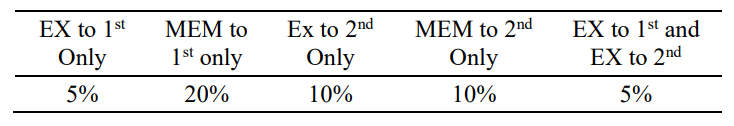
\includegraphics[width=0.5\linewidth]{figs/screenshot001}
\setRTL

فرض می‌کنیم درصد دستوراتی که وابستگی دارند مطابق جدول فوق است، پس برای هر نوع از دستورات تعداد چرخه تاخیر را محاسبه می‌کنیم	و سپس با فرض این که هیچ
$Forwarding$
ای نداریم، تسریع را حساب می‌کنیم:

\setLTR
$
\begin{cases}
	EX \ to \ 1st \ Only = 2 Delay Cycle \\
	MEM \ to \ 1st \ Only =2 Delay Cycle \\
	EX \ to \ 2nd \ Only = 1 Delay Cycle\\ 
	MEM \ to \ 2nd \ Only =1 Delay Cycle\\
	EX \ to \ 1st = 2 Delay Cycle\\
	EX \ to \ 2nd =  2 Delay Cycle
	\end{cases}
$

$
SpeedUp = \frac{T_1}{T_2} = \frac{\frac{CPI_1}{CR_1}}{\frac{CPI_2}{CR_2}} =
 \frac{\frac{5}{2.5}}{
\frac{0.05\times3 + 0.2\times3+0.1\times2+0.1\times2+0.05\times3+ 0.5\times1}{2}
} \simeq 2.2
$
\setRTL


\subsubsection*{ج}

اگر داده‌ها را به صورت زودهنگام در اختیار داشته باشیم باید فقط برای وابستگی 
$MEM \ to \ 1st \ only$
1 کلاک به تاخیر کنیم. پس:

\setLTR
$
SpeedUp = \frac{T_1}{T_2} = \frac{\frac{CPI_1}{CR_1}}{\frac{CPI_2}{CR_2}} = \frac{\frac{5}{2.5}}{\frac{0.2\times2 + 0.8\times1}{2}} = \frac{10}{3} 
\simeq 3.3
$
\setRTL

\subsubsection*{د}

در این صورت برای محاسبه شرط Branch باید یک چرخه Stall داشته باشیم. پس:

\setLTR
$
SpeedUp = \frac{T_1}{T_2} = \frac{\frac{CPI_1}{CR_1}}{\frac{CPI_2}{CR_2}} = \frac{\frac{5}{2.5}}{\frac{0.2\times2 + 0.1\times2+0.7\times1}{2}} \simeq 3.1
$
\setRTL

\pagebreak

\subsubsection*{ه}

اگر همه پرش‌ها را انجام نشده فرض کنیم، آن‌وقت تسریع برابر است با:

\setLTR
$
SpeedUp = \frac{T_1}{T_2} = \frac{\frac{CPI_1}{CR_1}}{\frac{CPI_2}{CR_2}} = \frac{5}{0.2\times2+0.1\times(0.2\times1+0.8\times2)+0.7\times1} \times \frac{2}{2} \simeq 3.12
$
\setRTL



\pagebreak


\مسئله{‌}
\subsubsection*{الف}

مقدار CPI را بدست می‌آوریم:

\setLTR
$
CPI = baseCPI + \sum missRate\times missPenalty = 2 + 0.1 \times 100 + 0.02 \times 0.4 \times 100 = 12.8
$
\setRTL

\subsubsection*{ب}
مقدار CPI جدید را بدست می‌آوریم:

\setLTR
$
CPI = 2 + 0.1 \times 10 + 0.04 \times 100 + 0.02 \times 0.4 \times 100 = 7.8
$
\setRTL
\pagebreak

\مسئله{‌}
در ابتدا تعداد بلوک‌ها را بدست می‌آوریم:

\setLTR
$
\frac{1MB}{16Byte} = \frac{2^{20}}{16\times8} = 2^{13} 
$
\setRTL

طول هر بلوک 16 بایت و 4 بیت مربوط به offset و 10 بیت برای برچسب‌ها داریم. پس تعداد بیت مربوط به index برابر است با:

\setLTR
$
24-4-10 = 10bit
$
\setRTL

چون ما $2^{13}$ بلوک و $2^{10}$ مجموعه داریم، پس درنتیجه 8 بلوک در هر مجموعه داریم. درنتیجه تعداد بیت‌های لازم در هر بلوک برابر است با:

\setLTR
$
16\times8+10+1 = 139 bits
$
\setRTL

پس تعداد کل بیت‌ها برابر است با:

\setLTR
$
n = 2^{13} \times139 = 1138688bits
$
\setRTL

اگر این حافظه associative fully باشد، بیت index نداریم و 20 بیت برای برچسب خواهیم داشت. حال دوباره تعداد بیت‌های هر بلوک را محاسبه می‌کنیم:

\setLTR
$
16\times8 + 20 + 1 =149bits \longrightarrow n = 2^{13} \times 149 = 1220608bits
$
\setRTL

اگر این حافظه mapping direct باشد، 13 بیت index داریم و 7 بیت برای برچسب خواهیم داشت. حال دوباره تعداد بیت‌های هر بلوک را محاسبه می‌کنیم:

\setLTR
$
16\times8 + 7 + 1 =136bits \longrightarrow n = 2^{13} \times 136 = 1114112bits
$
\setRTL

















\pagebreak

\مسئله{‌}
ترتیب اولیه دستورات به این صورت است:

\setLTR
\begin{lstlisting}
I1:     lw      R1, 0(R2)       ; R1 ← Memory[R2]
I2:     addi    R1, R1,     1   ; R1 ← R1+1
I3:     sw      R1, 0(R2)       ; Memory[R2] ← R1
I4:     addi    R2, R2,     8   ; R2 ← R2+8
I5:     addi    R4, R4,     -1  ; R4 ← R4-1
I6:     bne     R4, R0,     I1  ; branch if R4!=0
\end{lstlisting}
\setRTL

\subsubsection*{الف}
باید جایگاه
$I_5$
را طوری تغییر بدهیم که حداقل 2 مرحله زودتر از 
$I_6$
اجرا شود.

\setLTR
\begin{lstlisting}
I1:     lw      R1, 0(R2)       ; R1 ← Memory[R2]
I2:     addi    R1, R1,     1   ; R1 ← R1+1
I5:     addi    R4, R4,     -1  ; R4 ← R4-1
I3:     sw      R1, 0(R2)       ; Memory[R2] ← R1
I4:     addi    R2, R2,     8   ; R2 ← R2+8
I6:     bne     R4, R0,     I1  ; branch if R4!=0
\end{lstlisting}
\setRTL

البته در بخش‌های بعدی مجبور هستیم که جای دستورات 
$I2 , I5$
را تعویض کنیم چون در بخش بعدی فاصله آن کمتر از 2 می‌شود.

\subsubsection*{ب}
در این بخش ما دستوری را بعد از 
$I_6$
قرار می‌دهیم که هر بار اجرا شود و ارتباطی با شرط پرش نداشته باشد.

\setLTR
\begin{lstlisting}
I1:     lw      R1, 0(R2)       ; R1 ← Memory[R2]
I5:     addi    R4, R4,     -1  ; R4 ← R4-1
I2:     addi    R1, R1,     1   ; R1 ← R1+1
I3:     sw      R1, 0(R2)       ; Memory[R2] ← R1
I6:     bne     R4, R0,     I1  ; branch if R4!=0
I4:     addi    R2, R2,     8   ; R2 ← R2+8
\end{lstlisting}
\setRTL

\subsubsection*{ج}

با توجه به خواسته سوال، جدول زیر را تشکیل می‌دهیم:
\setLTR

$ \ \ 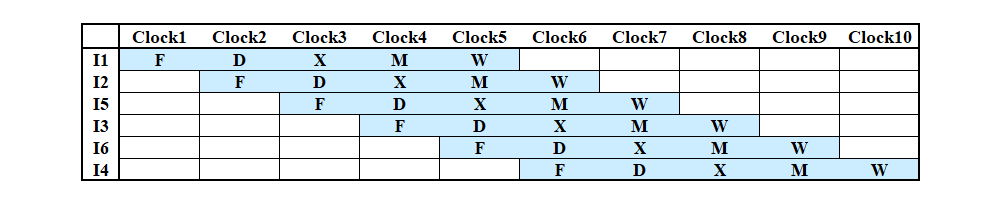
\includegraphics[width=1\linewidth]{figs/1.png}$

\setRTL

اگر فقط یک بار این حلقه اجرا شود، در مجموع 10 کلاک زمان می‌برد، اما اگر چندین بار این حلقه تکرار شود، تقریبا به تعداد حلقه‌ها نیاز به کلاک داریم.




\pagebreak
\end{document}